\section{Hand-made Data Structures}
\begin{frame}
  \begin{center}
    {\large Lecture 02 -- Data Structures\\Part IV -- Hand-made Data Structures}\\
  \end{center}
\end{frame}

\subsection{Motivation}
\begin{frame}
  \frametitle{Hand-making Data Structures}

  \begin{itemize}
  \item Sometimes, it is necessary to extend the standard data structures
    (arrays, maps, etc)
    \bigskip

  \item Other times, it is necessary to implement data structures not
    included in the standard libraries (graphs, UFDS, etc)
    \bigskip

  \item Let's see a few examples.
  \end{itemize}
\end{frame}

\subsection{Union-Find}
\begin{frame}
  \frametitle{Union-Find Disjoint Set (UFDS)}
  \framesubtitle{Motivating Problem}

  \begin{block}{Network Connections -- UVA793}
    In a network with $n$ computers, some are connected to others.\\
    \bigskip

    {\bf Input:} A series of ``commands''
    \begin{itemize}
    \item c i j -- Means computer $i$ is connected to computer $j$
    \item q i j -- Question: is computer $i$ connected to computer $j$?
    \end{itemize}

    \bigskip

    {\bf Output:} The number of ``q'' with answer yes, and the number
    of ``q'' with answer no.

  \end{block}
\end{frame}

\begin{frame}
  \frametitle{Union-Find Disjoint Set (UFDS)}
  \framesubtitle{Motivating Problem -- Naive answer}

  \begin{itemize}
  \item One idea: Use a Neighborhood Matrix $(n\times n)$ initalized with zeros.
  \item For every ``c i j'', $N_{i,j}, N_{j,i}$ becomes 1.
  \item We can follow the graph to answer ``q i j''.
  \end{itemize}

  \bigskip

  How good is this solution?
  \begin{itemize}
  \item Cost to insert a new connection: O(1)
  \item Cost to check if ``q i j'': O(n) (worst case)
  \end{itemize}

  \bigskip We can do better!
\end{frame}

\begin{frame}
  \frametitle{Union-Find Disjoint Set}

  \begin{center}
    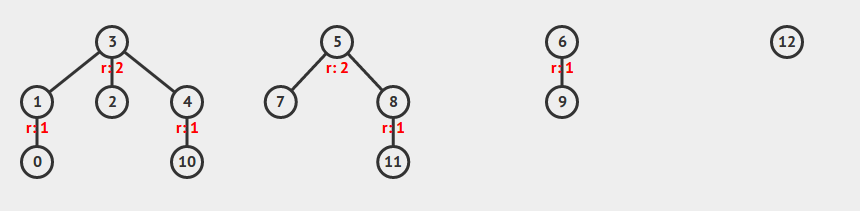
\includegraphics[width=.9\textwidth]{img/ufds1}
  \end{center}

  \begin{itemize}
  \item The UFDS keeps \structure{sets of items}, each is represented by a \structure{parent};
  \item When you join two sets \structure{You join their parents};
  \item When you test the parent of an item \structure{You flatten the tree};
  \item Test\_item and Join\_item are both O(1);
  \item More Information \url{https://visualgo.net/ja/ufds};
  \end{itemize}
\end{frame}

\begin{frame}[fragile]
  \frametitle{UFDS Implementation using Arrays}

  {\small
\begin{verbatim}
int p[MAX], r[MAX];
int find(int x) {
    return x == p[x] ? x : p[x]=find(p[x]);
}
int join(int x, int y) {
    x = find(x), y = find(y);
    if(x != y) {
        if(r[x] < r[y])
            p[x] = y, r[y] += r[x];
        else
            p[y] = x, r[x] += r[y];
        return 1;
    }
    return 0;
}
void init() {
    for(int i = 0; i < MAX; i++)
        p[i] = i, r[i] = 1; }

\end{verbatim}
}

\end{frame}

\begin{frame}
  \frametitle{Union Find Disjoint Set}
  \framesubtitle{Problem II -- War}
  {\small
  \begin{block}{}
    From a set of 10k people, some are friends, other are enemies.
    \begin{itemize}
      \item If A,B are friends, and B,C are friends, then A,C are friends
      \item If A,B are friends, and B,C are enemies, then A,C are enemies
      \item If A,B are enemies, and B,C are enemies, then A,C are friends
    \end{itemize}

    {\bf Input:} A series of commands from the set below:
    \begin{itemize}
    \item SetFriends(i,j)
    \item SetEnemies(i,j)
    \item TestFriends(i,j)
    \item TestEnemies(i,j)
    \end{itemize}

    {\bf Output:}
    \begin{itemize}
    \item If a ``SetFriends'' or ``SetEnemies'' is impossible, output ``-1''
    \item For a ``TestFriends'', ``TestEnemies'', output 0 - false, 1 - true
    \end{itemize}
  \end{block}}

\end{frame}

\begin{frame}
  \frametitle{Union Find Disjoint Set}
  \framesubtitle{Problem II -- War}

  This problem is similar to ``Networking'', but now you need to keep
  track of {\bf TWO} relations.

  \bigskip

  Some ideas:
  \begin{itemize}
  \item Keep UFDS for friends, and UFDS for enemies?
  \item Keep an ``enemy'' flag for each person?
  \item Add ``negative people'' to friend-set on UFDS?
  \end{itemize}

  \bigskip

  Which idea is easier to implement?
\end{frame}

\subsection{Segment Tree}
\begin{frame}[fragile]
  \frametitle{Range Maximum Query -- RMQ}

  Suppose you have an array of values:
\begin{verbatim}
Value: 18 17 13 19 15 11 20
Index:  0  1  2  3  4  5  6
\end{verbatim}

\bigskip

The \structure{Range Maximum Query} problem asks you to \structure{find
the index with the maximum value} between two indexes:

\begin{itemize}
  \item RMQ(0,0) = 0
  \item RMQ(0,6) = 6
  \item RMQ(1,4) = 3
\end{itemize}

\bigskip

\alert{Naive Method:} loop from $i$ to $j$, find maximum value. ($O(nk)$)\\
\medskip

But what is the number of {\bf Values} or {\bf Queries} is too big?
\end{frame}

\begin{frame}
  \frametitle{Segment Tree}

  \begin{itemize}
    \item Basic idea: \structure{index the array data in a binary tree}
    \bigskip

    \item Creation of the tree: \structure{$O(n)$}
    \bigskip

    \item Query of a segment: \structure{$O(\log n)$}
    \bigskip

    \item Update of the tree: \structure{$O(\log n)$} \hfill \alert{Important Part}
    \bigskip

    \item Many Implementations\\(this implementation: vector based heap)
  \end{itemize}
\end{frame}

\begin{frame}
  \frametitle{Segment Tree}
  \begin{center}
    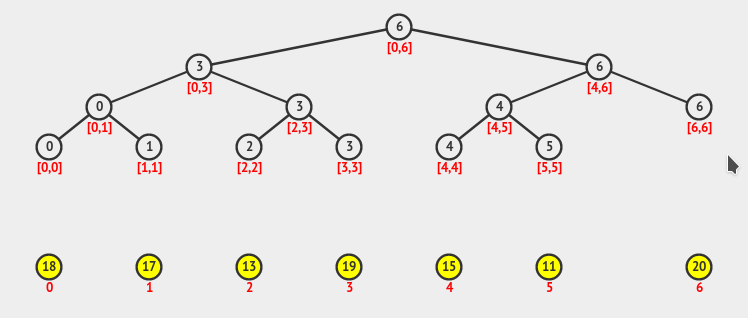
\includegraphics[width=1\textwidth]{img/segment_tree}
  \end{center}

  \bigskip

  Let's see the segment tree animation at VISUALGO.
\end{frame}

\begin{frame}[fragile]
  \frametitle{Coding the Segment Tree}
  \framesubtitle{Creating the Tree}
{\smaller
\begin{block}{}
\begin{verbatim}
typedef vector<int> vi; // We always use this!

class SegmentTree { // OOP implementation,
private: vi st, A;  // vi: typedef vector<int> vi;
  int n;
  int left (int p) { return  p<<1; }  // heap-like index;
  int right(int p) { return (p<<1) + 1; }

  void build(int p, int L, int R) {   // O(n log n)
    if (L == R)
      st[p] = L;                      // store the index
    else {                            // recursive build
      build(left(p) , L          , (L+R)/2);
      build(right(p), (L+R)/2 + 1, R      );
      int p1 = st[left(p)], p2 = st[right(p)];
      st[p] = (A[p1] <= A[p2]) ? p1 : p2;
  } }
\end{verbatim}
\end{block}}

\hfill\footnotesize{Code from \url{https://github.com/stevenhalim/cpbook-code}}

\end{frame}

\begin{frame}[fragile]
  \frametitle{Coding the Segment Tree}
  \framesubtitle{Query the Tree}
{\smaller
\begin{block}{rmq(1, 0, n-1, i, j) -- Query from i to j.}
\begin{verbatim}
int rmq(int p, int L, int R, int i, int j) // O(log n)
{
  if (i >  R || j <  L)
    return -1;    // outside query range
  if (L >= i && R <= j)
    return st[p]; // inside query range

  // compute the min position in the left and right part
  int p1 = rmq(left(p) , L        , (L+R)/2, i, j);
  int p2 = rmq(right(p), (L+R)/2+1, R      , i, j);

  if (p1 == -1) return p2;   // segment outside query
  if (p2 == -1) return p1;   // segment outside query
  return (A[p1] <= A[p2]) ? p1 : p2;
}
\end{verbatim}
\end{block}}
\hfill\footnotesize{Code from \url{https://github.com/stevenhalim/cpbook-code}}
\end{frame}

\begin{frame}[fragile]
  \frametitle{Coding the Segment Tree}
  \framesubtitle{Update the Tree}

{\smaller
\begin{block}{update(1, 0, n-1, i, v) -- update index i to value v}
\begin{verbatim}
int update(int p, int L, int R, int idx, int new_value) {
  int i = idx, j = idx;    //for point update i = j = idx
  // if the curr interval does not intersect the update,
  if (i > R || j < L) return st[p];  //return node value!
  // if the current interval is in the update range,
  if (L == i && R == j) {
    A[i] = new_value;     // update the underlying array
    return st[p] = L;     // this index
  }
  // compute the min pos in L/R part of the interval
  int p1, p2;
  p1=update(left(p) , L        , (L+R)/2, idx, new_value);
  p2=update(right(p), (L+R)/2+1, R      , idx, new_value);
  // return the position where the overall minimum is
  return st[p] = (A[p1] <= A[p2]) ? p1 : p2;
}
\end{verbatim}
\end{block}}
\hfill\footnotesize{Code from \url{https://github.com/stevenhalim/cpbook-code}}

\end{frame}
